\subsection{Scalability of NetShaper in Supporting Parallel Clients}
\label{subsec:netshaper-evaluation-num-clients}

To measure the number of clients NetShaper can support, we fix the request rate at 330k req/s (less than 10\% below server saturation rate), and spread this request rate across multiple clients, spawned by wrk2.
We increase the number of clients until we either observe some clients failing or we observe the latency increase by more than twice that of the latency observed with 330k clients in the experiment outlined in \Cref{subsec:netshaper-evaluation-http-reqs}.
As shown in \Cref{fig:netshaper-eval-parallel-clients}, NetShaper is able to sustain the same number of clients as the end application (Nginx).

\begin{figure}[!htb]
    \centering
    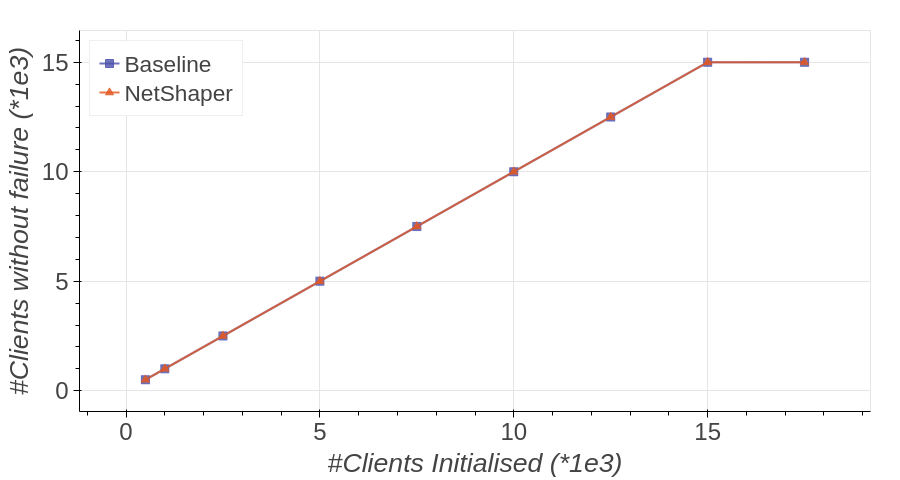
\includegraphics[width=\columnwidth]{figures/netshaper/evaluation/num_clients.png}
    \caption{NetShaper scalability with parallel clients}
    \label{fig:netshaper-eval-parallel-clients}
\end{figure}